

\chapter{Benchmarking of Non-blocking IO Processing Algorithms}
\label{cha:a_short_latex_tutorial_with_examples}

In this chapter, we delve into the benchmark results of two key algorithms applied using various strategies and implementations. These algorithms can be understood as abstract representations of real-world tasks that involve processing large amounts of data asynchronously. The two main algorithms under consideration are:

The main tasks can be broadly divided into two operations:

\begin{enumerate}
\item Finding the largest word in a set of files
\item Grouping of words based on their sizes, known as the "group words" operation
\end{enumerate}

The "group word" operation identifies words within a specified size range in a dataset. The algorithm then returns a collection of these words, along with a count of their occurrences, and is particularly designed to output the most recurring words within the specified range. This operation presents an intriguing computational challenge as it requires efficient data retrieval, processing, and frequency analysis.

Conversely, finding the largest word in a set of files, although seemingly simple, becomes a non-trivial task when considering vast amounts of data.

The data used in these tests is a collection of text files from Project Gutenberg, a large digital library of thousands of free eBooks. Project Gutenberg offers a wide variety of books in different languages, and for this experiment, we used a random sample of hundreds of books, providing a diverse and challenging dataset for our implementations.

To give a better idea of the operations, we present the pseudocode for each operation:


For the "group words" operation:

\begin{verbatim}
FUNCTION GroupWords(folder, minLength, maxLength)
    Create an empty map 'wordMap'
    FOR each file in 'folder' DO
        Skip the first 14 lines of the file (These are typically metadata in Gutenberg project files)
        FOR each remaining line in 'file' DO
            IF the line contains "*** END OF" THEN
                Break (This is the end of the actual content in Gutenberg project files)
            END IF
            FOR each word in 'line' DO
                IF length of 'word' is between 'minLength' and 'maxLength' THEN
                    Increment the count of 'word' in 'wordMap'
                END IF
            END FOR
        END FOR
    END FOR
    RETURN 'wordMap'
END FUNCTION

\end{verbatim}

For finding the largest word:


\begin{verbatim}
FUNCTION FindLargestWord(folder)
    Set 'largestWord' as an empty string
    FOR each file in 'folder' DO
        Skip the first 14 lines of the file (These are typically metadata in Gutenberg project files)
        FOR each remaining line in 'file' DO
            IF the line contains "*** END OF" THEN
                Break (This is the end of the actual content in Gutenberg project files)
            END IF
            FOR each word in 'line' DO
                IF length of 'word' is greater than length of 'largestWord' THEN
                    Set 'largestWord' as 'word'
                END IF
            END FOR
        END FOR
    END FOR
    RETURN 'largestWord'
END FUNCTION
\end{verbatim}

During the implementations, a conscious effort was made to keep the operation pipelines as similar as possible across the different technologies for each algorithm. This endeavor aimed to create a fair and representative evaluation of the behaviors of each technology. By maintaining consistency in pipeline operations, we can more accurately attribute performance differences to the underlying technology, rather than variations in the implemented code. This approach brings us closer to a true comparison of how each technology handles the challenges of asynchronous I/O data retrieval and processing.

In certain instances, particularly with Java, there was a need to incorporate external libraries for non-blocking asynchronous file retrieval. This requirement highlights the varying degrees of native support for these operations across programming environments. Some environments have native functions, while others rely heavily on third-party solutions. This aspect of the project mirrors the challenges often faced in real-world environments, where the necessity to adapt and find suitable solutions is a common part of the development process.

The implementations differ in the specific programming languages, libraries, and technologies they use. This allows us to evaluate the relative strengths and weaknesses of each approach and provides valuable insights into how these factors can affect performance.

After presenting and discussing each implementation and its results, we will be able to directly compare them. This will enable us to draw meaningful conclusions about the performance of the strategies and technologies when applied to the same task under the same conditions. Specifically, we are interested in how the performance of a given strategy or technology can vary across different programming frameworks when tasked with finding the largest word and executing the group word operation.

%\section{Strategies}
%\label{subsec:strategies}
%
%In this work were used various strategies implemented across different languages and technologies, some of those we already discussed in charpter \ref{cha:users_manual}. While some of these strategies can be used universally across all platforms, others are platform-specific due to the constraints of the environment.
%Bellow, you will find a brief enumeration of the strategies used,
%
%\subsection{Baseline}
%\label{subsubsec:baseline}
%The Baseline strategy is a straightforward implementation without any pipelining or other overhead. It serves as a reference for comparison. This method may use traditional synchronous I/O operations and sequential processing.
%
%These strategies will be applied to our chosen algorithms and implemented in the .NET, Java, and Kotlin environments. It's important to note that the aim is not to find the 'best' strategy but to demonstrate the relative strengths and weaknesses of each approach, how they can affect performance, and how they fit into different programming paradigms.
%
%\subsection{Asynchronous Baseline}
%\label{subsubsec:baseline}
%The "Asynchronous Baseline" strategy refers to a standard implementation of the baseline algorithm but using non-blocking IO operations. E.g. using async/await in C\# IO operation but without the pipeline operations.
%
%\subsection{Reactive Extensions (Rx)}
%\label{subsubsec:rx}
%Reactive Extensions (Rx) as discussed in charpter two. This model promotes a focus on data streams and the propagation of change. In the ambit of this work, were made implementations in several three programming environments, namely: .NET (Rx.NET), Java (RxJava), and JavaScript (RxJS).
%
%\subsection{Reactor (Flux)}
%\label{subsubsec:reactor_flux}
%As explained in charpter two, Reactor is a fourth-generation reactive library, based on the Reactive Streams specification, for building non-blocking applications on the JVM based on Java 8 and later. The Flux class, a Reactive Streams Publisher with reactive operators, emits 0 to N elements, and then completes (successfully or with an error). 
%This strategy will be benchmark using JAVA.
%
%\subsection{Streams}
%\label{subsubsec:blocking_reader_streams}
%This strategy uses Java's streams interface to read the data in a blocking manner. Due to the blocking nature of the I/O operations, this approach may lead to slower processing times as it has to wait for each I/O operation to complete.
%
%\subsection{Multi-threading}
%\label{subsubsec:multithread}
%This strategy leverages multi-threading to process data concurrently. By distributing the work across multiple threads, it often results in improved performance, especially for CPU-bound tasks.
%
%\subsection{Kotlin Flow}
%\label{subsubsec:kotlin_flow}
%Kotlin Flow, will be employed in our Java environment testing.
%
%\subsection{LINQ}
%\label{subsubsec:linq}
%For our .NET environment, among other technologies, we will utilize LINQ (Language Integrated Query), a Microsoft .NET Framework component adding native data querying capabilities to .NET languages.
%
%\subsection{IxJS}
%\label{subsubsec:ixjs}
%As explained in charpter two, in JS one of the technologies used will be IxJS, or Interactive Extensions for JavaScript.


\clearpage

\section{.NET Benchmarking}
\label{sec:dotnet_implementation}

In this subsection, we focus on the benchmark using different strategies in .NET programming environment.



\subsection{Find biggest word  results}
\label{subsubsec:biggest_word_results_cs}

For the find biggest word algorithm, are used the following strategies:

\begin{itemize}
    \item \textbf{Sync Baseline}: This strategy serves as the basic approach for finding the biggest word and acts as a baseline for comparison.
    \item \textbf{Async Baseline }: This strategy uses a single asynchronous task to find the biggest word.
    \item \textbf{Multithread }: A multi-threading approach that uses asynchronous blocking read operations.
    \item \textbf{Linq Sync}: This strategy uses Language Integrated Query (LINQ) in a synchronous manner.
    \item \textbf{Async Enumerable}: This approach uses asynchronous programming with enumerable collections.
    \item \textbf{RxNet}: The Reactive Extensions (Rx) library is used to handle data sequences asynchronously and event-based.
    \item \textbf{RxNet Async File Read}: This strategy uses the Reactive Extensions (Rx) library with asynchronous file reading operations.
\end{itemize}


In the following graphic, we have the results in seconds for each strategie:

%\begin{table}[H]
%    \centering
%    \resizebox{\textwidth}{!}{%
%    \begin{tabular}{|l|c|}
%    \hline
%    \textbf{Strategy} & \textbf{Processing Time Average (s)} \\ \hline
%    Sync Baseline & 15.8 \\ \hline
%    Multithread  & 1.6 \\ \hline
%    Async Baseline & 2.8 \\ \hline
%    Linq Sync & 22.2 \\ \hline
%    Async Enumerable & 30 \\ \hline
%    Rx & 23 \\ \hline
%    Rx Async File Read & 15 \\ \hline
%    \end{tabular}%
%    }
%    \caption{Processing times for different strategies for "Find the biggest word".}
%    \label{tab:biggest_word_results_cs_1}
%\end{table}
    
\begin{figure}[H]
    \raggedright
    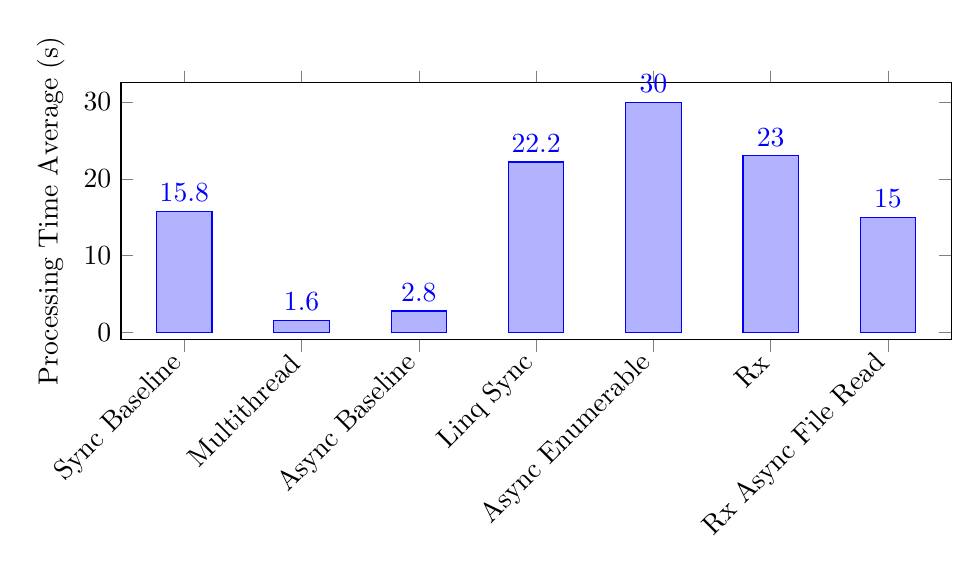
\begin{tikzpicture}
    \begin{axis}[
    ybar=2*\pgflinewidth,
    width=1.0\textwidth,
    height=0.4\textwidth,
    bar width=20pt,
    enlargelimits=0.09,
    legend style={at={(0.5,-0.2)}, anchor=north, legend columns=-1},
    ylabel={Processing Time Average (s)},
    symbolic x coords={Sync Baseline, Multithread, Async Baseline, Linq Sync, Async Enumerable, Rx, Rx Async File Read},
    xtick=data,
    xticklabel style={rotate=45,anchor=east},
    nodes near coords,
    nodes near coords align={vertical},
    ]
    \addplot coordinates {(Sync Baseline, 15.8) (Multithread, 1.6) (Async Baseline, 2.8) (Linq Sync, 22.2) (Async Enumerable, 30) (Rx, 23) (Rx Async File Read, 15)};
    \end{axis}
    \end{tikzpicture}
    \caption{Processing times for different strategies for "Find the biggest word".}
    \label{fig:biggest_word_results_cs_2}
\end{figure}

\clearpage


\subsection{Group Word Results}
\label{subsubsec:group_word_processing_times_cs}

In this subsection, we concentrate on the task of grouping words from a file using different strategies. The strategies that we evaluate here include:

\begin{itemize}
    \item \textbf{Baseline}: This strategy serves as the basic approach for word grouping and acts as a baseline for comparison.
    \item \textbf{Linq}: A synchronous approach that handles tasks in a sequential manner.
    \item \textbf{AsyncEnumerable}: This strategy uses .NET asyncenumerables to process the asynchronous data .
    \item \textbf{RxNet}: Here, the Reactive Extensions (Rx) library is used to handle data sequences asynchronously and event-based.
\end{itemize}


%\begin{table}[H]
%    \centering
%    \resizebox{\textwidth}{!}{%
%    \begin{tabular}{|l|c|}
%    \hline
%    \textbf{Strategy} & \textbf{Processing Time Average (s)} \\ \hline
%    Baseline Blocking IO & 26 \\ \hline
%    Linq & 22 \\ \hline
%    Async Enumerable & 30 \\ \hline
%    Rx Net & 22 \\ \hline
%    \end{tabular}%
%    }
%    \caption{Processing times for different strategies for "Count Words".}
%    \label{tab:group_word_processing_times_cs}
%\end{table}

\begin{figure}[H]
    \raggedright
    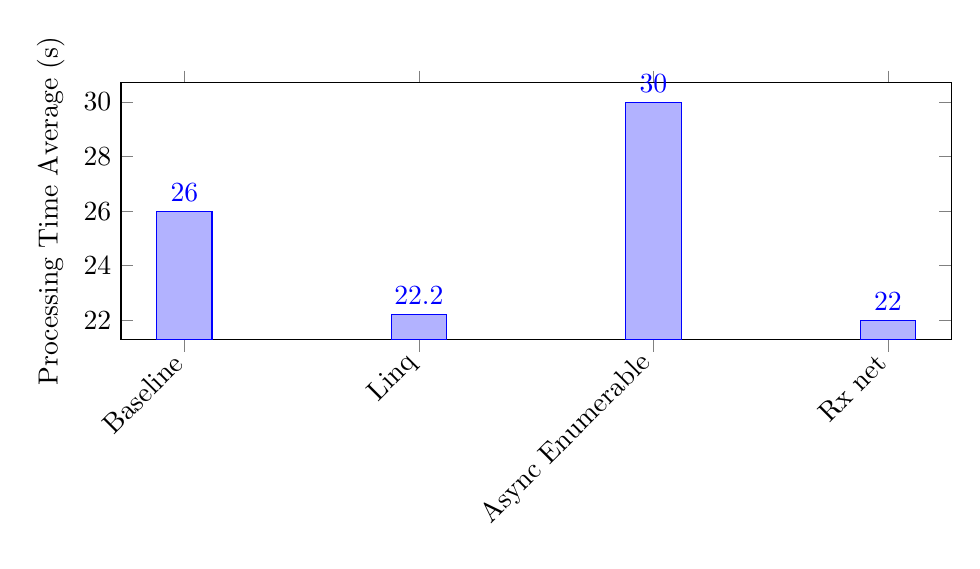
\begin{tikzpicture}
    \begin{axis}[
        ybar=2*\pgflinewidth,
        width=1.0\textwidth,
        height=0.4\textwidth,
        bar width=20pt,
        enlargelimits=0.09,
        legend style={at={(0.5,-0.2)}, anchor=north, legend columns=-1},
        ylabel={Processing Time Average (s)},
        symbolic x coords={Baseline, Linq, Async Enumerable, Rx net},
        xtick=data,
        xticklabel style={rotate=45,anchor=east},
        nodes near coords,
        nodes near coords align={vertical},
        ]
    \addplot coordinates {(Baseline, 26.0) (Linq, 22.2) (Async Enumerable, 30) (Rx net, 22.0)};
    \end{axis}
    \end{tikzpicture}
    \caption{Processing times for different strategies for "Count Words".}
    \label{fig:group_word_processing_times_cs}
\end{figure}


\clearpage

\section{Java/Kotlin Benchmarking}
\label{sec:java_implementation}

In this section, we explore and assess diverse strategies applied in Java and Kotlin to process files, and we scrutinize their performances solving the "Find Word" an "Group Word algorithms"


\subsection{Biggest Word Results}
\label{subsubsec:biggest_word_results}

The strategies used in JAVA are:

\begin{itemize}
    \item \textbf{Baseline}: This strategy illustrates a basic non-blocking I/O operation, serving as a comparison baseline.
    \item \textbf{Flux}: These strategies leverage the Reactor Flux model from Java's Project Reactor library. The former follows a standard non-concurrent processing model, while the latter introduces parallelization for improved performance.
    \item \textbf{RXJava}: This strategy employ the RXJava library. They replace the Reactor Flux with Observables, with the distinction being made between non-concurrent and concurrent processing.
    \item \textbf{Streams, MultiThread, and Streams with Paralelism}: These strategies use Java's Streams API and explore handling of blocking operations under three different conditions: standard usage, with multithreading, and with concurrency within streams.
    
\end{itemize}


In the following graphic, we have the results in seconds for each strategy:

%\begin{table}[H]
%    \centering
%    \resizebox{\textwidth}{!}{%
%    \begin{tabular}{|l|c|}
%    \hline
%    \textbf{Strategy} & \textbf{Processing Time Average (s)} \\ \hline
%    NIO Reactor Flux & 1.1\\ \hline
%    NIO Reactor Flux with Concurrency (use of \texttt{parallel()}) & 1.0 \\ \hline
%    NIO Observable RXJava & 0.9 \\ \hline
%    NIO Observable with Concurrency (use of \texttt{parallel()})& 0.8 \\ \hline
%    Blocking Reader in Streams & 3.9 \\ \hline
%    Blocking Reader MultiThread  & 0.7 \\ \hline
%    Blocking Reader Streams with Concurrency & 3.0 \\ \hline
%    NIO Baseline & 0.9 \\ \hline
%    Concurrent Processing with Kotlin Flow & 2.4 \\ \hline
%    Sequential Processing with Kotlin Flow & 5.1 \\ \hline
%    Kotlin Flow IO Blocking Operations & 5.2 \\ \hline
%    \end{tabular}%
%    }
%    \caption{Processing times for different Java/Kotlin strategies for "Biggest Word".}
%    \label{tab:strategies_times_biggest_word}
%\end{table}
    
   
    \begin{figure}[H]
        \raggedright
        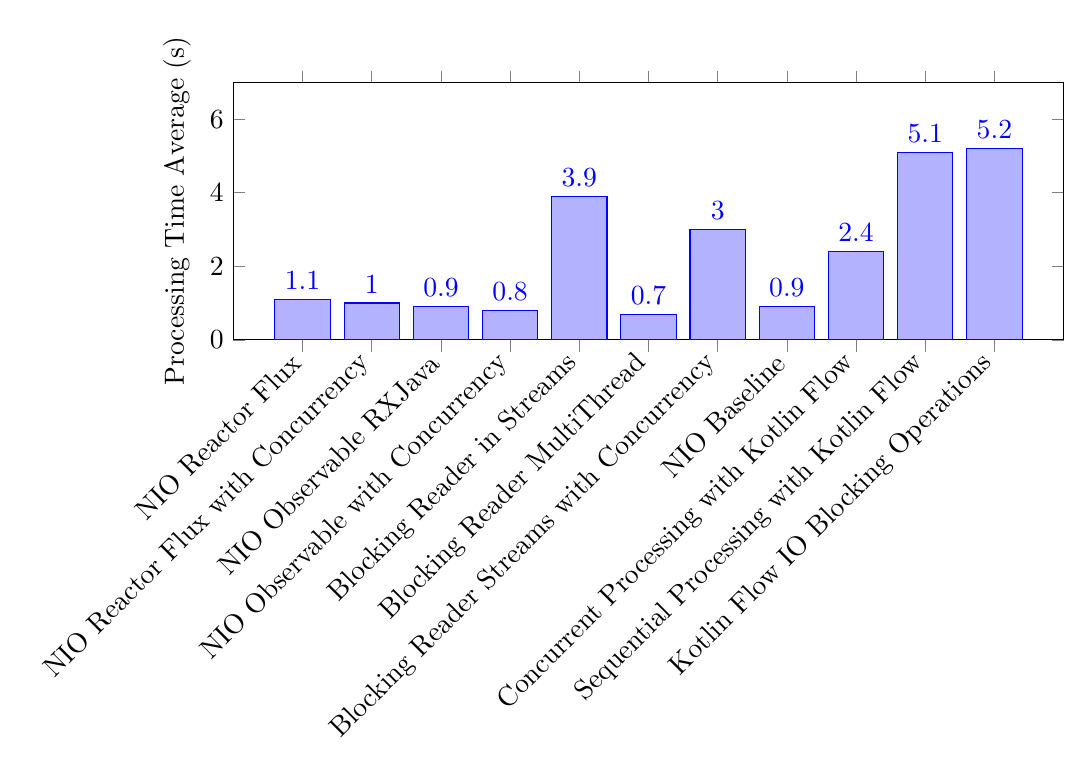
\begin{tikzpicture}
        \begin{axis}[
            ybar=2*\pgflinewidth,
            width=1.0\textwidth,
            height=0.4\textwidth,
            bar width=20pt,
            legend style={at={(0.5,-0.2)}, anchor=north, legend columns=-1},
            ylabel={Processing Time Average (s)},
            symbolic x coords={NIO Reactor Flux, NIO Reactor Flux with Concurrency, NIO Observable RXJava, NIO Observable with Concurrency, Blocking Reader in Streams, Blocking Reader MultiThread, Blocking Reader Streams with Concurrency, NIO Baseline, Concurrent Processing with Kotlin Flow, Sequential Processing with Kotlin Flow, Kotlin Flow IO Blocking Operations},
            xtick=data,
            xticklabel style={rotate=45,anchor=east},
            nodes near coords,
            nodes near coords align={vertical},
            ymin=0, ymax=7,
            ]
        \addplot coordinates {(NIO Reactor Flux, 1.1) (NIO Reactor Flux with Concurrency, 1.0) (NIO Observable RXJava, 0.9) (NIO Observable with Concurrency, 0.8) (Blocking Reader in Streams, 3.9) (Blocking Reader MultiThread, 0.7) (Blocking Reader Streams with Concurrency, 3.0) (NIO Baseline, 0.9) (Concurrent Processing with Kotlin Flow, 2.4) (Sequential Processing with Kotlin Flow, 5.1) (Kotlin Flow IO Blocking Operations, 5.2)};
        \end{axis}
        \end{tikzpicture}
        \caption{Processing times for different Java/Kotlin strategies for "Biggest Word".}
        \label{fig:biggest_word_processing_times}
    \end{figure}
    

    \clearpage

    \subsection{Group Word Results}
    \label{subsubsec:group_word_results}
    
   The strategies discussed here include:

    \begin{itemize}
        \item \textbf{Baseline}: This strategy serves as a baseline for comparison. It illustrates a basic non-blocking I/O operation without the use of any high-level constructs like Reactor Flux or Observable.
        \item \textbf{RXJava}: This strategy employs the RXJava library, popular for building asynchronous and event-driven applications.
        \item \textbf{Flux}: This strategy leverages the Reactor Flux model available in Java's Project Reactor library, providing an efficient approach to handling asynchronous data sequences.
        \item \textbf{MultiThread}: This strategy uses Java's Streams API and explores handling of blocking operations with the help of multi-threading.
        \item \textbf{Streams}: Similar to the previous strategy, this one uses Java's Streams API, but handles blocking operations within streams.
        \item \textbf{Flow (Kotlin)}: This strategy utilizes Kotlin's Coroutines and Flow API, which are particularly well-suited for handling multiple values that are emitted sequentially.
    \end{itemize}

    In the following table and graphic, we have the results in seconds for each strategy:

%\begin{table}[H]
%        \centering
%        \resizebox{\textwidth}{!}{%
%        \begin{tabular}{|l|c|}
%        \hline
%        \textbf{Strategy} & \textbf{Processing Time Average (s)} \\ \hline
%        Baseline & 1.3 \\ \hline
%        RXJava & 5.8 \\ \hline
%        Reactor Core Flux & 12.0 \\ \hline
%        Blocking IO W MultiThread & 1.2 \\ \hline
%        Streams & 1.8 \\ \hline
%        Flow (Kotlin) & 15.0\\ \hline
%        \end{tabular}%
%        }
%        \caption{Processing times for different Java/Kotlin strategies for "Group Words".}
%        \label{tab:strategies_times_group_words}
%    \end{table}
        
    \begin{figure}[H]
        \centering
        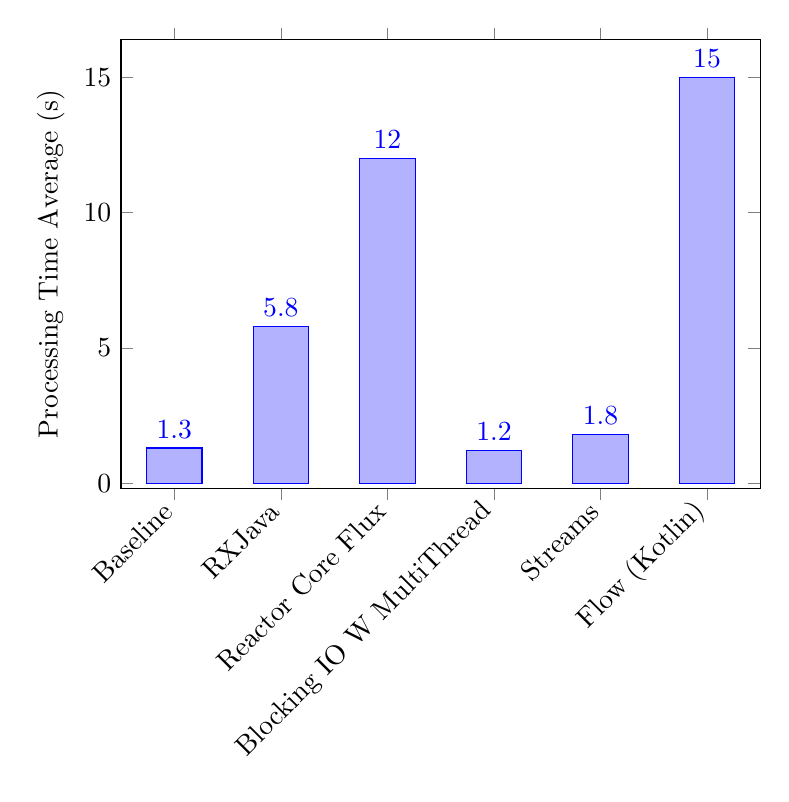
\begin{tikzpicture}
        \begin{axis}[
            ybar=2*\pgflinewidth,
            width=0.8\textwidth,
            height=0.6\textwidth,
            bar width=20pt,
            legend style={at={(0.5,-0.2)}, anchor=north, legend columns=-1},
            ylabel={Processing Time Average (s)},
            symbolic x coords={Baseline, RXJava, Reactor Core Flux, Blocking IO W MultiThread, Streams, Flow (Kotlin)},
            xtick=data,
            xticklabel style={rotate=45,anchor=east},
            nodes near coords,
            nodes near coords align={vertical},
            ]
            \addplot coordinates { (Baseline, 1.3) (RXJava, 5.8) (Reactor Core Flux, 12.0) (Blocking IO W MultiThread, 1.2) (Streams, 1.8) (Flow (Kotlin), 15.0)};
        \end{axis}
        \end{tikzpicture}
        \caption{Processing times for different Java/Kotlin strategies for "Group Words".}
        \label{fig:processing_times}
    \end{figure}
    

    \clearpage
... 
% Here you conclude the entire chapter by summarizing your findings and interpretations.


\section{JavaScript Benchmarking}
\label{sec:js_implementation}


\subsection{Finding the Biggest Word}
\label{subsec:biggest_word_js}

Here, we investigate the following four (to add ixjs) strategies:

\begin{itemize}
    \item \textbf{Baseline for await..of without pipeline}: This strategy serves as the basic JavaScript approach for finding the biggest word, acting as a baseline for comparison.
    \item \textbf{Baseline for await..of with pipeline}: This strategy uses JavaScript streams, which provide a way to handle reading/writing files, network communications, or any kind of end-to-end information exchange in an efficient manner.
    \item \textbf{RxJS}: This strategy leverages the Reactive Extensions for JavaScript (RxJS) library, which offers a set of methods for dealing with asynchronous data sequences in an effective way.
\end{itemize}


In the following graphic, we have the results in seconds for each strategie:

%\begin{table}[H]
%    \centering
%    \resizebox{\textwidth}{!}{%
%    \begin{tabular}{|l|c|}
%    \hline
%    \textbf{Strategy} & \textbf{Processing Time Average (s)} \\ \hline
%    Baseline JS & 8.2 \\ \hline
%    Baseline Stream JS & 23.2 \\ \hline
%    RxStrategy JS & 13.9 \\ \hline
%    \end{tabular}%
%    }
%    \caption{Processing times for different JavaScript strategies for "Biggest Word".}
%    \label{tab:strategies_times_biggest_word_js}
%\end{table}

\begin{figure}[H]
    \raggedright
    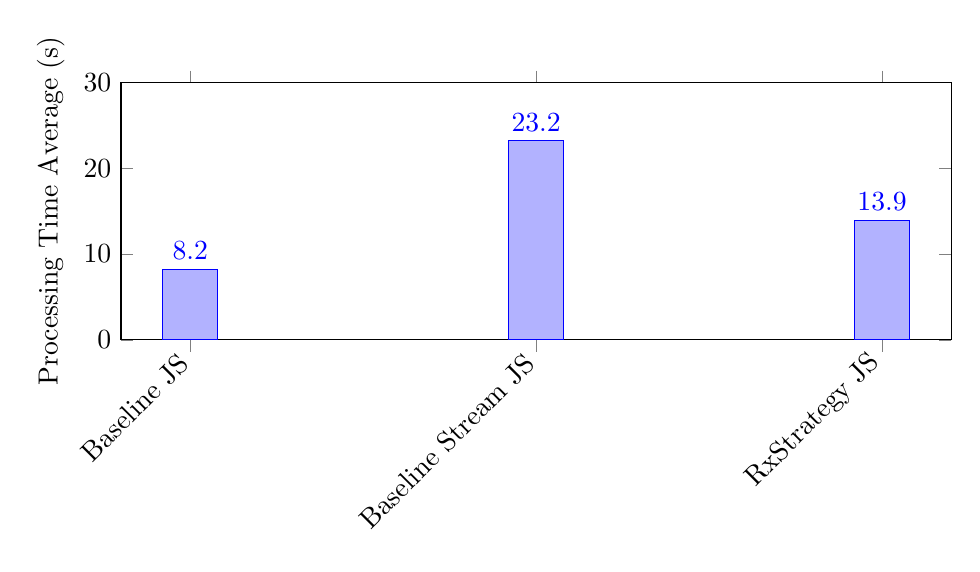
\begin{tikzpicture}
    \begin{axis}[
        ybar=2*\pgflinewidth,
        width=1.0\textwidth,
        height=0.4\textwidth,
        bar width=20pt,
        legend style={at={(0.5,-0.2)}, anchor=north, legend columns=-1},
        ylabel={Processing Time Average (s)},
        symbolic x coords={Baseline JS, Baseline Stream JS, RxStrategy JS},
        xtick=data,
        xticklabel style={rotate=45,anchor=east},
        nodes near coords,
        nodes near coords align={vertical},
        ymin=0, ymax=30,
        ]
    \addplot coordinates {(Baseline JS, 8.2) (Baseline Stream JS, 23.2) (RxStrategy JS, 13.9)};
    \end{axis}
    \end{tikzpicture}
    \caption{Processing times for different JavaScript strategies for "Biggest Word" Graphic}
    \label{fig:biggest_word_processing_times_js}
\end{figure}

\clearpage


\subsection{Grouping Words}
\label{subsec:grouping_words_js}

In this subsection, we evaluate the following strategies for grouping words:

\begin{itemize}
    \item \textbf{Baseline JS}: This strategy serves as the basic JavaScript approach for grouping words, acting as a baseline for comparison.
    \item \textbf{Baseline Stream JS}: This strategy uses JavaScript streams, which provide a way to handle reading/writing files, network communications, or any kind of end-to-end information exchange in an efficient manner.
    \item \textbf{RxStrategy JS}: This strategy leverages the Reactive Extensions for JavaScript (RxJS) library, which offers a set of methods for dealing with asynchronous data sequences in an effective way.
\end{itemize}

In the following graphic, we present the results in seconds for each strategy:

%\begin{table}[H]
%    \centering
%    \resizebox{\textwidth}{!}{%
%    \begin{tabular}{|l|c|}
%    \hline
%    \textbf{Strategy} & \textbf{Processing Time Average (s)} \\ \hline
%    Baseline JS & 30.1 \\ \hline
%    Baseline Stream JS & 26.6 \\ \hline
%    RxStrategy JS & 17.3 \\ \hline
%    \end{tabular}%
%    }
%    \caption{Processing times for different JavaScript strategies for "Grouping Words".}
%    \label{tab:strategies_times_grouping_words_js}
%\end{table}

\begin{figure}[H]
    \raggedright
    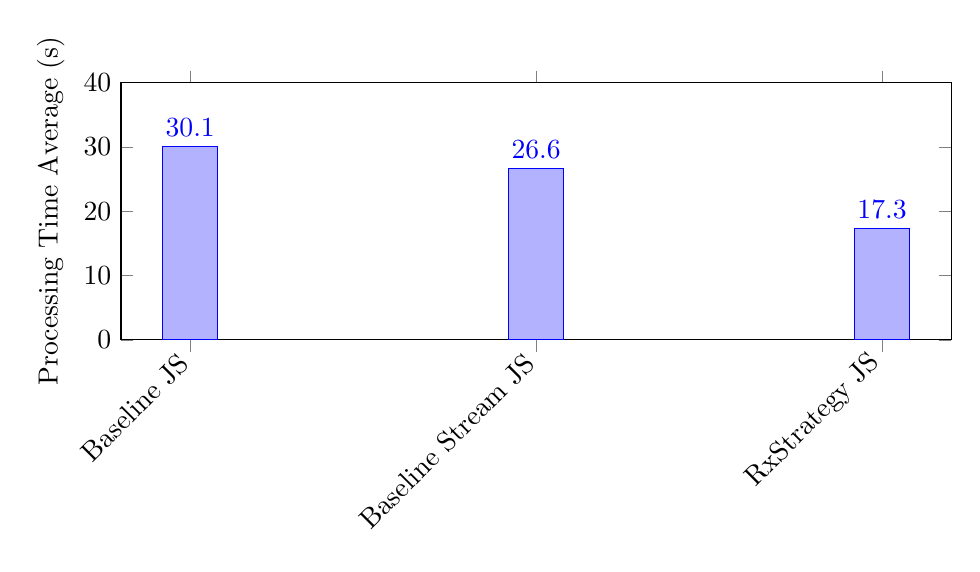
\begin{tikzpicture}
    \begin{axis}[
        ybar=2*\pgflinewidth,
        width=1.0\textwidth,
        height=0.4\textwidth,
        bar width=20pt,
        legend style={at={(0.5,-0.2)}, anchor=north, legend columns=-1},
        ylabel={Processing Time Average (s)},
        symbolic x coords={Baseline JS, Baseline Stream JS, RxStrategy JS},
        xtick=data,
        xticklabel style={rotate=45,anchor=east},
        nodes near coords,
        nodes near coords align={vertical},
        ymin=0, ymax=40,
        ]
    \addplot coordinates {(Baseline JS, 30.1) (Baseline Stream JS, 26.6) (RxStrategy JS, 17.3)};
    \end{axis}
    \end{tikzpicture}
    \caption{Processing times for different JavaScript strategies for "Grouping Words" Graphic}
    \label{fig:grouping_words_processing_times_js}
\end{figure}



\clearpage



\section{Conclusions}
\label{subsec:discussion}

TO ask: Results discussion to be made in previous subsection? Here just for main conclusions? 



\end{document}